% \begin{itemize}
%     \item Network connectivity, E/I balance, raster plots
%     \item Too many possible connections to test them all → Subsampling
%     \item Performance of last chapter's methods
%     \item If time: experiment with a network that is less densely connected than our current fully-random one. Why? To better examine the effect of indirect connections / colliders (For the current connectivity, there are too many of those. But in a more realistic, 'localized' network, there are less, and so it seems easier to isolate and examine their effect).
% \end{itemize}

\section{Introduction}

In the previous experiments, only one neuron's voltage was simulated. The inputs were Poisson spike trains.
In the next experiments, we simulate the voltages of a full network of neurons, which are recurrently connected to each other.
The goal is to investigate the effect on network inference of potentially correlated inputs and indirect connections.




\section{Connectivity structure}

\begin{figure}
    \subfloat{
        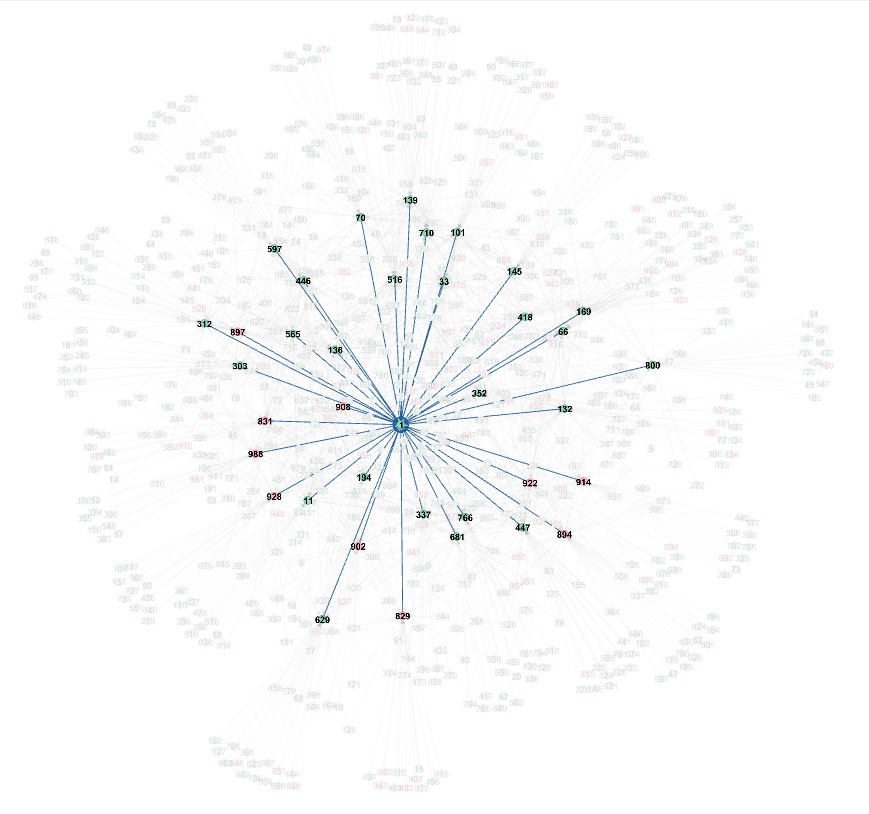
\includegraphics[w=0.75]{gephi-direct-inputs.png}
        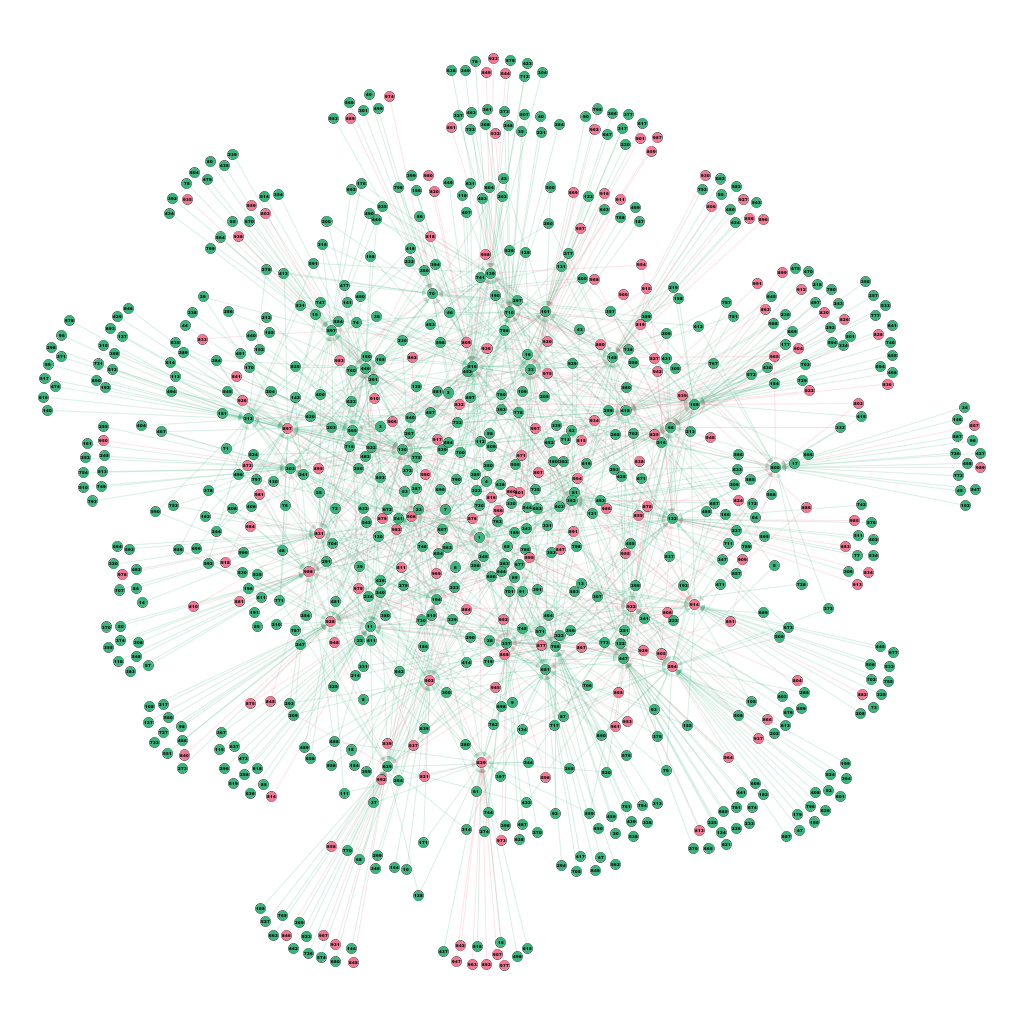
\includegraphics[w=0.75]{gephi-inputs-to-inputs.png}
    }
    \vspace*{2em}
    \caption
        {\textbf{A neuron is reachable in two hops from most other neurons}.    Selected neurons and connections in our random network. Left shows the direct inputs to one of the neurons. Right additionally shows the direct inputs to these inputs. This subnetwork already contains more than 700 of the 1000 total neurons in the network.\\
        Excitatory neurons in green, inhibitory in red. The tangle in the middle consists of neurons that synapse onto multiple of the direct inputs of our selected neuron.\\
        Visualization using the `Gephi' software, with the `Yifan-Hu' layout algorithm, and default parameters otherwise.
        Source: \nburl{2022-08-29__Visualizing_subnets}.}
    \label{fig:gephi-network-viz}
\end{figure}

% These two margin figs can go to Appendix
\marginpar{
    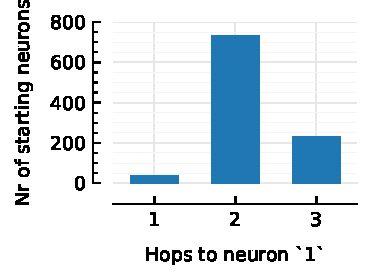
\includegraphics[w=1, trim={0 0.4em 0 -1em}, clip]{shortest-path-1}
    \captionof{figure}{
        \textbf{A selected neuron is reachable in at most three hops.}
        Shortest path lengths from every other neuron in the network.}
    \label{fig:shortest-path-1}
}
\marginpar{
    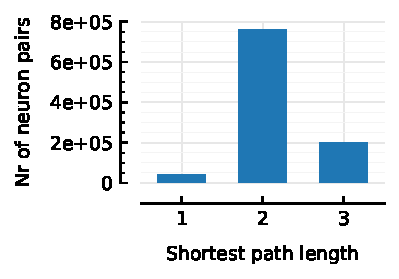
\includegraphics[w=1, trim={0 0.4em 0 -1em}, clip]{shortest-path-all}
    \captionof{figure}{
        \textbf{Every neuron is reachable in at most three hops.}
        Shortest path lengths calculated using the Floyd-Warshall algorithm. Source: \nburl{2022-07-14__Unconnected-but-detected.html}.}
    \label{fig:shortest-path-all}
}

We choose the simple and common `fully random' connectivity rule,\footnote{
    Other common choices for connectivity structure are scale-free networks, and `local' networks.
}
where any neuron has a connection to another with a uniform random probability (we choose $p_\text{conn} = 0.04$). After generating an adjacency matrix this way (\verb|A = rand(N, N) .≤ 0.04|, where \verb|rand| draws from $\sim U[0,1]$), we remove autapses. We choose the number of neurons $N = 1000$.

A property of fully random networks is that they are strongly interconnected. In our network, any neuron is reachable from any other in at most three steps (three synapses); most are reachable in just two. This is exemplified in \cref{fig:gephi-network-viz} and \cref{fig:shortest-path-1}: one selected neuron (neuron `1' here) is reachable in two hops from more than 700 of the 1000 total neurons in the network. And when we compute the shortest path between every possible neuron pair, we find a very similar distribution (\cref{fig:shortest-path-all}).




\section{External input}

As we no longer have Poisson spike trains providing input to our neurons, we need another way of bootstrapping activity in the network.\\
Instead of external spikes, each neuron is provided with external input by adding Gaussian noise to its membrane voltage. Every time step ($Δt = 0.1$~ms), a sample drawn from a normal distribution with mean $–0.5$~pA and $σ = 5$~pA is added to the membrane current. (As membrane current is by convention negative, this corresponds to an on-average positive influence on membrane voltage).\\
Like in the first footnote in \cref{sec:model-voltage-imaging}, this way of adding noise makes the noise power dependent on the timestep. A more principled approach to injecting noise would be to replace our ODE for the neuron voltage (\cref{eq:AdEx-V}) by a stochastic differential equation (SDE); though we did not explore this here.


\section{EI balance}

Similar to the N-to-1 experiments, we make 1 out of 5 neurons inhibitory.
As before, this is done by setting the synaptic reversal potential at the outputs of inhibitory neurons to $-80$ mV (instead of the $0$ mV for excitatory neurons).
To make sure that each neuron receives a balanced mix of excitation and inhibition, and given that there are 4:1 excitatory to inhibitory neurons, we make excitatory neurons 4x weaker: their synaptic strength ($Δg$, the instantaneous increase in postsynaptic conductance $g$ on spike arrival) is 4x as small as that of inhibitory neurons.

% Option for appendix, these four figs
\begin{figure}
    \subfloat{
        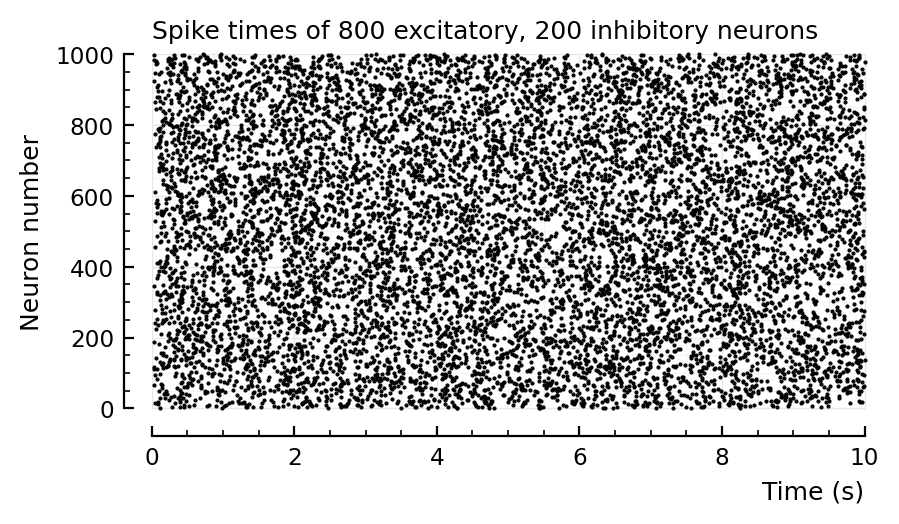
\includegraphics[w=0.74]{1144_raster}
        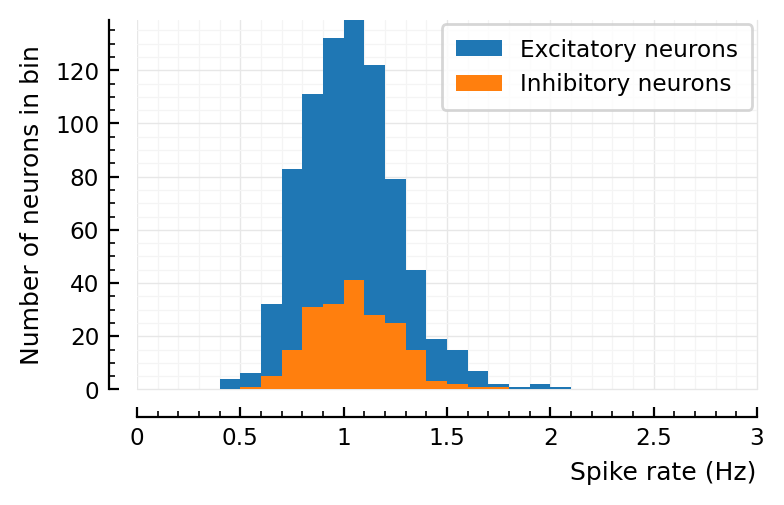
\includegraphics[w=0.74]{1144_hist}
    }
    \captionn
        {Firing rates in the network with `1144' weights}
        {Left: rasterplot showing all spikes in the first 10 seconds of the simulation.\\
        Right: histogram of firing rates.\\
        Source: \nburl{2022-07-01__g_EI}.}
    \label{fig:1144-weights}
\end{figure}

\begin{figure}
    \subfloat{
        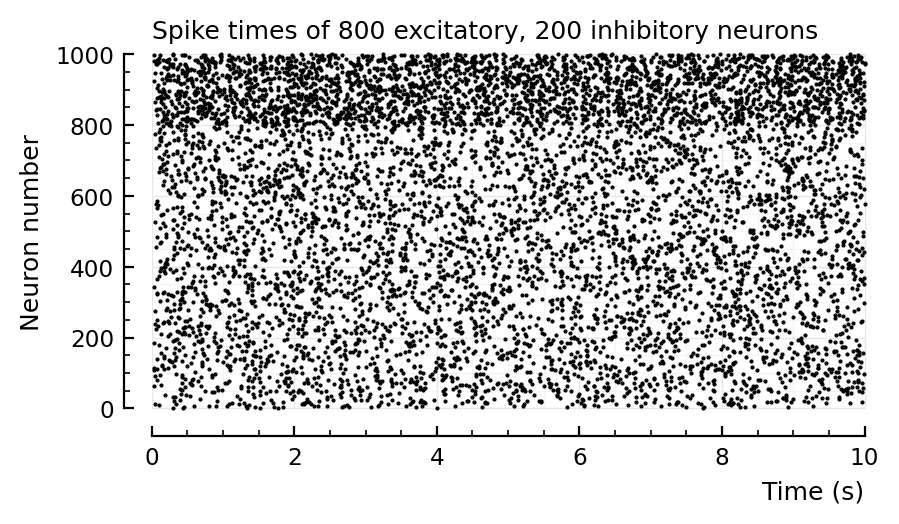
\includegraphics[w=0.74]{roxin_raster}
        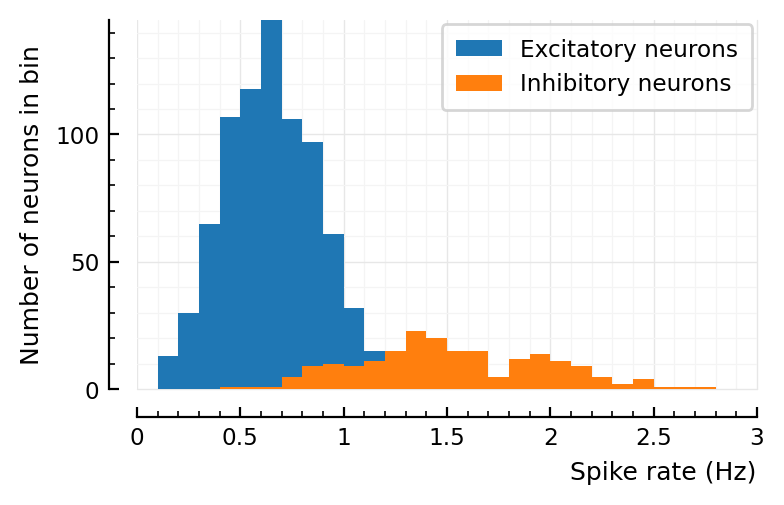
\includegraphics[w=0.74]{roxin_hist}
    }
    \captionn
        {Firing rates in the network with `Roxin2011' weights}
        {See \cref{fig:1144-weights}.}
    \label{fig:roxin-weights}
\end{figure}

% A synaptic weight rule where inhibitory synapses are 4× stronger to compensate for there being 4× as many synapses.
% Given that we simulated four times as many excitatory as inhibitory neurons, the synaptic weight rule described above (with inhibitory synapses 4× as strong) seems logical, to keep excitation and inhibition in balance.
\Cref{fig:1144-weights} shows results of the network simulation as spiketrains and firing rate distributions, using the described synaptic weights rule (inhibitory synapses 4× stronger than excitatory ones). We find that the resulting firing rate distribution is fairly symmetrical, and that excitatory and inhibitory neurons have very similar firing rates.

In real neural networks however, inhibitory neurons often have higher firing rates than their excitatory neighbours. In addition, real firing rate distributions are often heavy-tailed and not symmetrical, as we saw back in \cref{sec:lognormal-poisson-input}.
So, to coax more realistic firing rate distributions out of our network, we looked at the previously mentioned modelling paper of Roxin \emph{et al}, ``On the Distribution of Firing Rates in Networks of Cortical Neurons'', \cite{Roxin2011DistributionFiringRates}.\footnote{
    This paper seeks to explain how heavy-tailed firing rate distributions emerge in randomly connected spiking neural networks. We wanted to emulate the simulations in this work, to obtain a heavy-tailed firing rate distribution.
}
% Their figures indeed seem to show a lognormal-like distribution of firing rates from their simulatd networks.
In this paper different synaptic weights are used than the ones described above.
Normalizing excitatory-to-excitatory (\verb|E→E|) connections to 1, Roxin et al's synaptic weights are:
\begin{verbatim}
    E→E: 1
    E→I: 18 (instead of 1)
    I→E: 36 (instead of 4)
    I→I: 31 (instead of 4)
\end{verbatim}
We will call these weights `Roxin2011'. The naive, `balancing' weights used in \cref{fig:1144-weights}, we will call `1144'.

Simulating a network with the `Roxin2011' weights indeed increases the firing rates of inhibitory neurons with respect to those of excitatory neurons (\cref{fig:roxin-weights}). The two firing rate distributions are however both as symmetrical as before.\footnote{
    When collating the two firing rate distributions from both neuron types, the resulting single distribution \emph{is} heavy-tailed, and even vaguely looks log-normal (but it is not). In \cite{Roxin2011DistributionFiringRates}, similar-looking, collated firing rate distributions are shown, and are called lognormal (but this is never quantified in the paper).
}

This imbalance between \verb|E→E| and \verb|E→I| synapses is not that rare: another modelling paper that also investigated EI-balance, \cite{Sadeh2021ExcitatoryinhibitoryBalanceModulates}, has the following synaptic weights. If our original weights are $[1, 1, 4, 4]$, then Sadeh and Clopath's weights are $[1, k, k, k]$, with $k = 4$ (in their "strong E-I coupling regime").

In the results that follow, we use both `1144' and the `Roxin2011' synaptic weights.

Finally, we also looked at drawing synaptic weights from a distribution (specifically, a lognormal one) instead of setting all weights of one type to be equal. This did not change the symmetry of the resulting firing rate distributions, so we did not pursue this further.


\section{Subsampling}

We simulate all 1000 neurons' voltages, but, to save memory and disk space,  do not record all these traces.\footnote{
    For a 10-minute simulation with a timestep of 0.1 ms, one voltage trace takes 48 MB (at 64 bit per sample). Our 1000 neurons thus take 48 GB -- and that is just for one simulation (one set of parameters).\newline
    We \emph{do} record the spike trains of all neurons. Saving just spike times takes considerably less space: a neuron spiking at 10 Hz for 10 minutes emits 6000 spikes, which, at 64 bit per timestamp, takes just  48 kB.\newline
    In other words,  at a 0.1 ms sample rate, a spike train occupies about 1000× less memory than the corresponding voltage trace.
}
In most experiments here, we recorded the voltage traces of 40 excitatory and 10 inhibitory neurons (5\% of all neurons).

Additionally, when performing connection tests on the inputs of a recorded neuron, we do not test the spiketrains of all 999 other neurons. Instead, we test only a (biased) sample of the possible inputs, to save processing time.
This sample is constructed as follows. We test all the a-priori known true direct inputs -- both excitatory and inhibitory -- and add a random sample of 40 not-directly-connected neurons.

On average, each neuron has ± 32 excitatory inputs and ± 8 inhibitory inputs. This means that, from the 1000 × 1000 possible connections, we only test about 4000, or 0.4\%.\footnote{
    Calculation behind these numbers:\\
    - 1000 neurons × 80\% excitatory × 4\% probability of an input connection = 32 excitatory inputs on average.\\
    - 50 `post' neurons (40 excitatory and 10 inhibitory voltage-recorded neurons) × 80 `pre' neurons (±40 connected + 40 unconnected) = 4000 tested connections.\\
    - To be precise, instead of 1000 × 1000, there are rather  $1000^2 - 1000$ possible connections, as we would not test for autapses.
}

\begin{figure}
    \subfloat{
        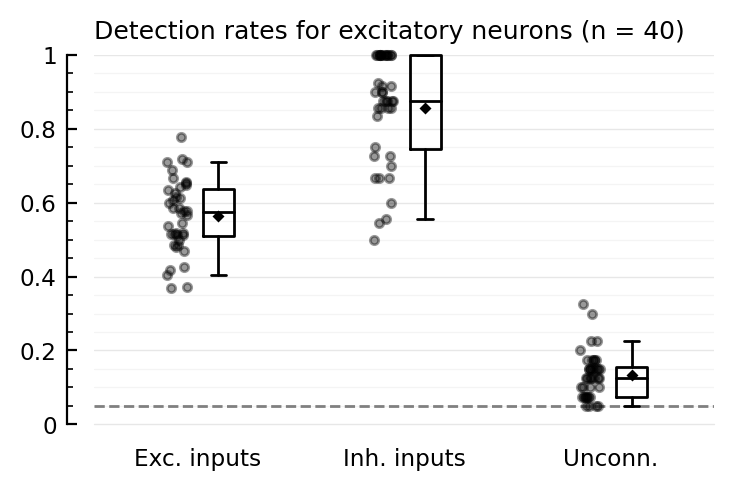
\includegraphics[w=0.74]{2022-09-01__1144_weights_23_0.png}
        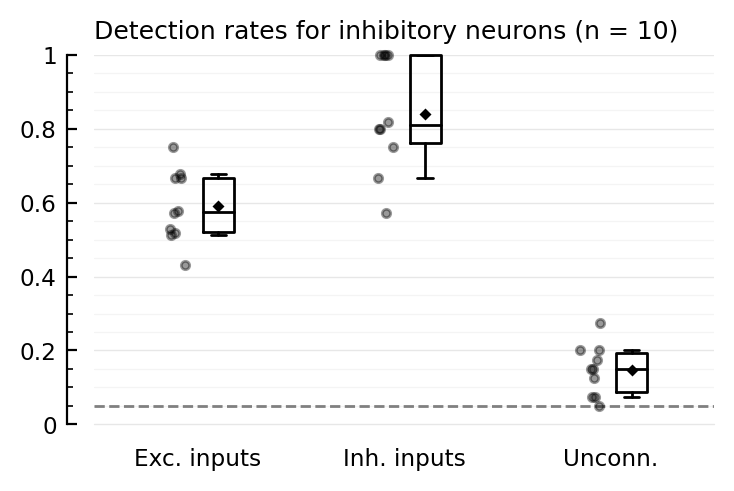
\includegraphics[w=0.74]{2022-09-01__1144_weights_24_0.png}
    }
    \captionn[. ]
    {Performance of the STA `peak-to-peak' connection test in the random network}
    {10 minute recording, with `1144' weights. Each dot is the true positive rate for one `post' neuron. The gray dotted line indicates the p-value threshold α of 0.05.\\
    Source: \nburl{2022-09-01__1144_weights}.}
    \label{fig:net-perf}
    \vspace*{2em}
\end{figure}



\section{Connection testing}

We tested connections using the STA height (or `peak-to-peak') test. In the chronology of the PhD, the more advanced methods presented in the previous chapter were developed only after the network tests in this chapter were done. Applying the newer methods to the full network (and not just the N-to-1 setup) is a topic for further work.
% also: detrates at fixed threshold, instead of AUC.

\Cref{fig:net-perf} shows the performance of using the STA height as connection test in the network. The detection rates (one for each tested `post' neuron and `pre' neuron type) are shown at a fixed detection threshold $α$ of $0.05$. That is, a connection was classified as real if its STA was larger than 95 of its 100 `control' STAs, which where made by randomly shuffling the presynaptic spiketrains.\footnote{
    A spiketrain is shuffled by taking its inter-spike-intervals (ISIs), randomly shuffling those, and reconstructing a new spiketrain from the resulting shuffled ISIs.
}

Detection rates are broken down per type of both the presynaptic and postsynaptic neuron (excitatory or inhibitory). We find that inhibitory inputs are significantly easier to detect (independent of the type of the postsynaptic neuron). This is due to the synaptic weight of inhibitory inputs -- and thus their PSPs -- being $4×$ stronger than those of excitatory inputs.

The most interesting category in \cref{fig:net-perf} are the `Unconnected' detection rates (i.e. the false positive rates, FPRs), which are almost all higher than the detection threshold $α$. In theory, the FPR should equal the detection threshold α; and indeed this is what we roughly found in the N-to-1 experiments with STA-height shuffle test.\footnote{
    This is true almost by definition of the shuffle test: an unconnected spiketrain in the N-to-1 experiment has randomly generated spiketimes. Shuffling this random spiketrain creates more random spiketrains. Looking at the distribution of STA heights of these random spiketrains, the chance that the `real' STA (of the unconnected spiketrain) is in the top-α fraction of STA heights -- and that thus, it would be wrongly classified as a true input, i.e. a false positive -- is exactly α.
}
In the network, we thus detect unconnected inputs -- or to be more precise: not-directly-connected inputs -- at a rate higher than chance. This deserves more scrutiny, which we do in the next section.



\section{False positive detections}

As a summary of the above: when we test unconnected spiketrains as inputs to some neuron in the network, we falsely classify them as connected at a higher rate than would be expected if these spiketrains were fully random. So, they have a stronger-than-random STA. Or in other words, their spikes seem to have some influence on the target neuron's voltage, even though they are not direct inputs to it. In this section, we examine what is special about these false positive input neurons.

First, we found that all false positives (i.e. all not-directly-connected inputs that were nonetheless classified as connected) had a shortest path to the target neuron that consisted of only one in-between neuron. However, as we saw in \cref{fig:shortest-path-all}, this is not that special in this highly-interconnected random network.

But maybe there are \emph{more} such length-2 paths between the input neuron and the target neuron? We indeed found that this was the case when examining one target neuron and all its tested unconnected inputs. In \cref{fig:net-FP} (left), the blue distribution (number of length-2 paths to the target neuron, for false positive inputs) is higher than the orange distribution (same, but for true negatives).

Next, we looked at the type of in-between neurons on the shortest path. We found that for the false positive inputs, the in-between neuron was more likely to be inhibory (\cref{fig:net-FP}, right). This makes sense, as inhibitory inputs are stronger (they are also detected at a higher rate, as seen in \cref{fig:net-perf}).

\begin{figure}
    \subfloat{
        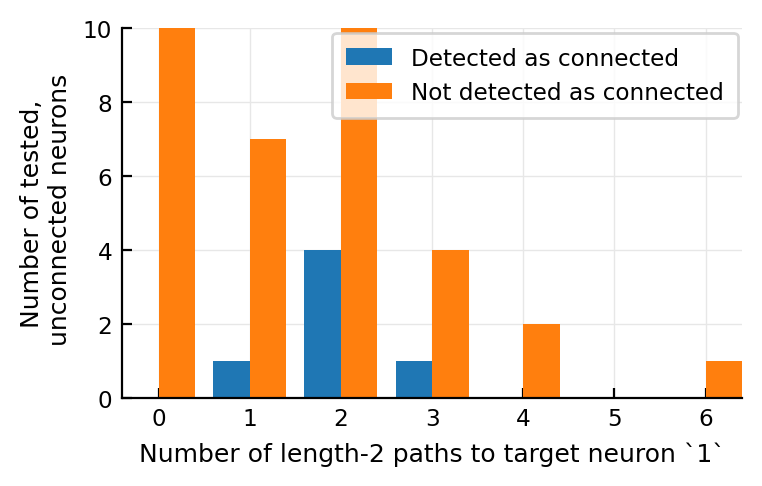
\includegraphics[w=0.74]{net-FP-length-2-paths}
        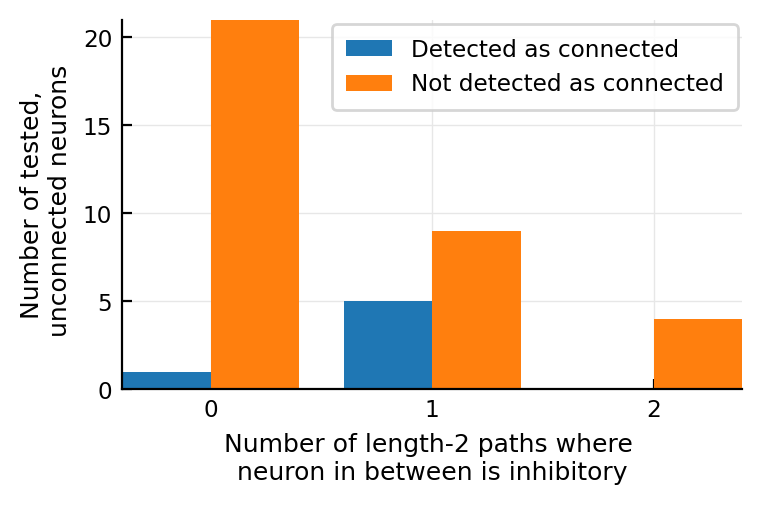
\includegraphics[w=0.74]{net-FP-inh}
    }
    \captionn
        {Characterizing what is different about false positive inputs}
        {All tested unconnected inputs to a selected target neuron in the network, with inputs correctly classfied as not-connected in orange, and the false positives in blue. Source: \nburl{2022-07-14__Unconnected-but-detected}.}
    \label{fig:net-FP}
    % \vspace*{2em} % to space from plot underneath.
\end{figure}


Finally, we looked at the firing rate of the in-between neurons (\cref{fig:net-FP-fr}). For false positives inputs, the in-between neurons were more active than for true negatives.


\begin{figure}
    \begin{sidecaption}
        {\textbf{False positives synapse onto high-firing direct inputs}.\\
        See \cref{fig:net-FP}.}
        [fig:net-FP-fr]
        \linelabel{fig:net-FP-fr}
        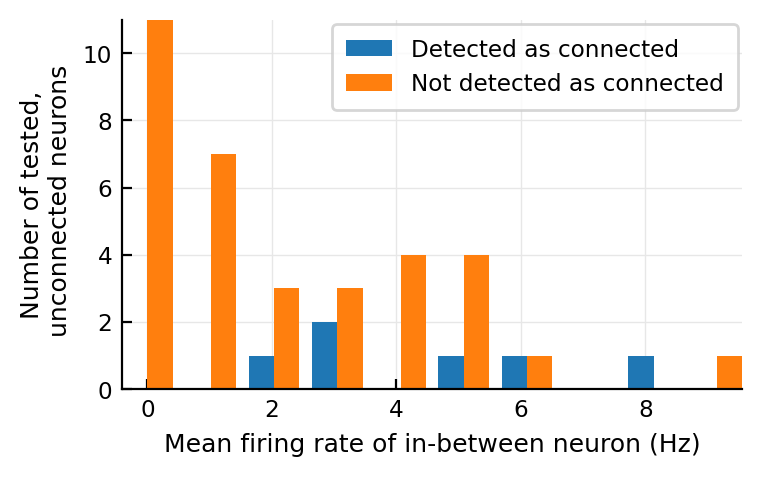
\includegraphics[w=0.74]{net-FP-fr}
    \end{sidecaption}
\end{figure}


% We tested spiketrain correlations as well: https://tfiers.github.io/phd/nb/2022-08-05__Spiketrain-correlations.html
% (but no signif difference, at any binsize)


In summary, we have some evidence (though it should be tested more thoroughly) that our higher-than-expected false positive rate is due to indirect inputs: neurons that synapse onto direct inputs. False positives synapse onto more such direct inputs, and those direct inputs have a stronger influence on the target neuron: a higher firing rate, and more likely to be inhibitory.

Further work could adapt our network topology to be more sparse, so that indirect connections are much rarer, and their effect easier to study.




\section{Conclusion}

In this chapter, we extended the N-to-1 testing setup to a full network of simulated neurons. We found that the STA height method could still detect connections. However, unlike in the N-to-1 setup -- with its fully independent inputs -- in the network, the false positive rate exceeded the detection threshold α. We hypothesized that this is due to indirect connections being detected as direct inputs, and found some preliminary evidence that that is indeed the case.

\marginpar{
    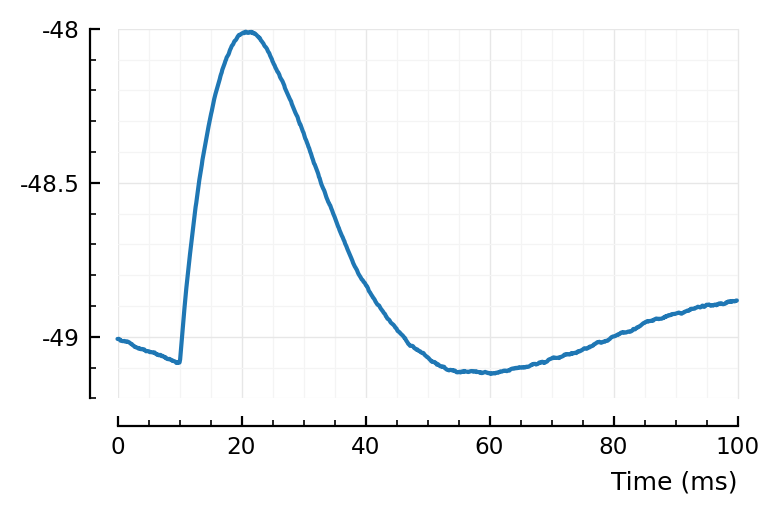
\includegraphics[w=1]{avg_STA}
    \captionof{figure}{
        Average STA of all true excitatory connections to recorded neurons in the network. Source: \nburl{2022-09-09__Conntest_with_template_matching}.
    }
    \label{fig:avg_STA}
}

One of the avenues pursued during the investigation of the indirect connections, was to plot their STA and compare it to the `ideal' STA\footnote{
    The hypothesis was that we would see a voltage bump twice as late as for direct connections, i.e. indicating a disynaptic connection. This investigation was inconclusive, but it did give us ideas for new connection detection methods.
}. This ideal STA (\cref{fig:avg_STA}) was made by using the ground truth connectivity and averaging all the STAs of the true direct connections. This clean STA gave us the idea to (1) model this shape, and use this model as some sort of `prior' for a stronger connection test; and (2) use it as a template to correlate STAs with. This led us to the new connection tests discussed in the next chapter.
